% banco_pruebas. GENERADO por pruebas_banco.py: no editar a mano.
\documentclass[border=0pt,tikz]{standalone}
\usepackage[utf8]{inputenc}
\usepackage[T1]{fontenc}
\usepackage{lmodern}
\usepackage[none]{hyphenat}
% Estilo común de las figuras TikZ (panoramas y diagramas de bloques).
%
% Cada figura lo incluye con \input{../../figuras/estilo_tikz.tex} (las figuras
% viven en docs/<módulo>/figuras/). Un solo lugar para la paleta, los estilos de
% bloque y el formato de los parámetros: si cambia algo acá, cambia en todas.
%
% La paleta es la misma de docs/figuras/estilo_svg.py y de PALETA en
% modulos/mk/datasheet.py; si se toca un color, se toca en los tres.
%
% Requiere: \usepackage{tikz} (lo da la clase standalone con la opción tikz).

\usetikzlibrary{arrows.meta,positioning,calc,fit,backgrounds,shapes.multipart,
                decorations.markings,shadows}

% ---------------------------------------------------------------- colores ---
\definecolor{azul}{RGB}{108,172,228}      % acondicionamiento
\definecolor{verde}{RGB}{110,214,142}     % captura / histogramas en BRAM
\definecolor{amarillo}{RGB}{252,232,160}  % trigger
\definecolor{naranja}{RGB}{252,206,160}   % camino a DDR
\definecolor{grisr}{RGB}{226,226,226}     % compartido / infraestructura
\definecolor{rojo}{RGB}{240,128,128}      % bus del sistema

% ---------------------------------------------------------------- estilos ---
\tikzset{
  >={Stealth[length=2.4mm,width=1.8mm]},
  % fondo blanco siempre: el SVG se ve igual en modo claro y oscuro
  fondo/.style   = {show background rectangle, inner frame sep=8pt,
                    background rectangle/.style={fill=white, draw=none}},
  bloque/.style  = {draw=black, line width=0.6pt, rounded corners=2pt,
                    align=center, text width=2.2cm, minimum height=1.15cm,
                    inner sep=2pt, font=\scriptsize, fill=#1},
  datos/.style   = {bloque=azul!35},
  trig/.style    = {bloque=amarillo},
  captura/.style = {bloque=verde!55},
  ddr/.style     = {bloque=naranja!70},
  comp/.style    = {bloque=grisr},
  bus/.style     = {bloque=rojo!45},
  % lógica escrita dentro del módulo, sin submódulo propio
  etapa/.style   = {bloque=#1, line width=0.5pt},
  etapa/.default = verde!20,
  % lo que el bitstream no trae (atado a cero, stub, salida muda)
  mudo/.style    = {bloque=white, draw=black!45, dashed, text=black!55},
  %
  % BLOQUE CON PARÁMETROS, en el formato del datasheet: el encabezado lleva el
  % nombre y los parámetros con que lo instancia el padre (NOMBRE=valor, en
  % monoespaciada, uno por línea); el cuerpo, más claro, lo que hace.
  %   \node[datos, param={azul!35}{azul!12}] {\blk{nombre}{} \prm{A=1\\B=2}
  %                                            \nodepart{two} función};
  param/.style 2 args = {rectangle split, rectangle split parts=2,
                         rectangle split part fill={#1, #2}},
  %
  flujo/.style   = {->, line width=0.8pt},
  ctrl/.style    = {->, line width=0.6pt, black!65},
  % la línea que pasa por encima en un cruce: un halo blanco la separa
  cruce/.style   = {preaction={draw=white, line width=3.4pt, -}},
  % marca de ancho de bus: barra oblicua a mitad de la flecha, con el número
  % encima. \draw[flujo, ancho=14] ...; para otra posición, ancho en=0.3.
  ancho/.style   = {decoration={markings, mark=at position \anchopos with {
                      \draw[line width=0.6pt, -] (-0.1,-0.14) -- (0.1,0.14);
                      \node[font=\scriptsize, above=1.5pt] {#1};}},
                    postaction={decorate}},
  % la misma marca en una flecha vertical: el número va a la derecha
  anchov/.style  = {decoration={markings, mark=at position \anchopos with {
                      \draw[line width=0.6pt, -] (-0.14,-0.1) -- (0.14,0.1);
                      \node[font=\scriptsize, right=3pt] {#1};}},
                    postaction={decorate}},
  ancho en/.code = {\def\anchopos{#1}},
  sen/.style     = {font=\scriptsize\ttfamily, inner sep=1.5pt},
  nodo/.style    = {font=\tiny\ttfamily, inner sep=1pt, black!75},
  pin/.style     = {font=\scriptsize, align=center, inner sep=1pt},
  grupo/.style   = {draw=black!55, dashed, line width=0.7pt, rounded corners=4pt},
  canal/.style   = {grupo},
  contenedor/.style = {draw=black!80, line width=1.0pt, rounded corners=6pt},
  % marca numerada: cada número es una fila de la tabla del documento
  marca/.style   = {circle, fill=black, text=white, font=\scriptsize\bfseries,
                    inner sep=0pt, minimum size=4.3mm},
  %
  % DECISIONES (docs/mca/vista_general_mca.md). Cada opción es un bloque, todas
  % entran a un mux (\muxdec, abajo) y el registro que elige entra por abajo.
  % la opción que trae el reset (el comportamiento histórico): borde doble
  defecto/.style = {double=white, double distance=0.8pt, line width=0.45pt},
  % rótulo de la decisión, el mismo Dn del panorama y del documento
  decision/.style = {circle, fill=black, text=white, font=\small\bfseries,
                     inner sep=0pt, minimum size=7mm},
  %
  % LÓGICA (docs/mca/figuras/contabilidad/ y los detalles de las decisiones)
  % registro: caja gris con el triángulo de reloj en el borde de abajo
  registro/.style = {draw=black, line width=0.6pt, fill=grisr, align=center,
                     font=\scriptsize, inner sep=2pt, minimum width=#1,
                     minimum height=0.85cm,
                     path picture={\draw[line width=0.5pt]
                       ([xshift=-1.1mm]path picture bounding box.south) --
                       ([yshift=1.6mm]path picture bounding box.south) --
                       ([xshift=1.1mm]path picture bounding box.south);}},
  registro/.default = 0.8cm,
  % condición de una cadena if / else-if: "sí" sale a la derecha, "no" abajo
  pregunta/.style = {draw=black, line width=0.5pt, rounded corners=7pt,
                     fill=white, font=\scriptsize\ttfamily, align=center,
                     inner sep=2.5pt, minimum height=0.62cm, text width=#1},
  pregunta/.default = 1.9cm,
  si/.style      = {font=\tiny, inner sep=1pt, above, pos=0.12},
  no/.style      = {font=\tiny, inner sep=1pt, left, pos=0.45},
  %
  titulo/.style  = {anchor=north west, font=\small, inner sep=4pt, align=left},
  rotulo/.style  = {anchor=north west, font=\scriptsize\itshape, black!70,
                    inner sep=2pt, align=left},
}

% submódulo: nombre en monoespaciada; lógica propia: nombre en romana
\newcommand{\blk}[2]{{\ttfamily\bfseries #1}\\[1pt]#2}
\newcommand{\etq}[2]{{\bfseries #1}\\[1pt]#2}
\newcommand{\punto}[1]{\fill (#1) circle (1.3pt);}

% Parámetros en el formato del datasheet: NOMBRE=valor en monoespaciada, una
% entrada por celda, hasta cuatro columnas. Una columna: \prm{A=1\\B=2};
% dos: \prm{A=1 & B=2\\C=3}.
\newcommand{\prm}[1]{{\ttfamily\fontsize{5.6}{6.6}\selectfont
  \begin{tabular}{@{}l@{\hspace{7pt}}l@{\hspace{7pt}}l@{\hspace{7pt}}l@{}}#1\end{tabular}}}

\def\anchopos{0.5}

% Mux de una decisión: trapecio con el lado ancho (las entradas) a la izquierda.
% #1 = nombre, #2 = centro, #3 = alto en cm. Deja tres coordenadas:
%   (#1-in)  centro del lado de entradas: las flechas llegan a (#1-in |- opcion.east)
%   (#1-out) la salida
%   (#1-sel) mitad del lado de abajo: por ahí entra el registro que elige
% El rótulo de adentro es opcional: \muxdec{m}{(4,0)}{3.6} y después
% \node[...] at (m) {...}.
\newcommand{\muxdec}[3]{%
  \path #2 coordinate (#1);
  \draw[line width=0.6pt, fill=grisr]
    ($(#1)+(-0.45,{#3/2})$) -- ($(#1)+(0.45,{#3/2-0.35})$) --
    ($(#1)+(0.45,{-#3/2+0.35})$) -- ($(#1)+(-0.45,{-#3/2})$) -- cycle;
  \coordinate (#1-in)  at ($(#1)+(-0.45,0)$);
  \coordinate (#1-out) at ($(#1)+(0.45,0)$);
  \coordinate (#1-sel) at ($(#1)+(0,{-#3/2+0.175})$);}

% El mismo mux rotado 90 grados, para un flujo de arriba hacia abajo: entradas
% por el lado ancho de arriba, salida abajo y el registro que elige por la
% izquierda. #1 = nombre, #2 = centro, #3 = ancho en cm. Deja (#1-in) centro del
% lado de entradas, (#1-out) la salida y (#1-sel) mitad del lado izquierdo.
\newcommand{\muxdecv}[3]{%
  \path #2 coordinate (#1);
  \draw[line width=0.6pt, fill=grisr]
    ($(#1)+({-#3/2},0.45)$) -- ($(#1)+({#3/2},0.45)$) --
    ($(#1)+({#3/2-0.35},-0.45)$) -- ($(#1)+({-#3/2+0.35},-0.45)$) -- cycle;
  \coordinate (#1-in)  at ($(#1)+(0,0.45)$);
  \coordinate (#1-out) at ($(#1)+(0,-0.45)$);
  \coordinate (#1-sel) at ($(#1)+({-#3/2+0.175},0)$);}

% Leyenda de colores + nota. #1 = posición, #2 = color/texto, #3 = nota.
\newcommand{\leyenda}[3]{%
  \begin{scope}[shift={(#1)}, every node/.style={font=\scriptsize}]
    \coordinate (t0) at (-0.5,0);
    \foreach \c/\t [count=\i] in {#2} {
      \pgfmathtruncatemacro\j{\i-1}
      \node[draw, fill=\c, minimum width=4mm, minimum height=3mm, inner sep=0pt,
            right=5mm of t\j.east, anchor=west] (l\i) {};
      \node[right=1.5mm of l\i] (t\i) {\t};
    }
    \node[anchor=north west, black!70, text width=19cm, align=left]
      at (-0.05,-0.3) {#3};
  \end{scope}}

% Lo que dicen los parámetros, para la nota de la leyenda
\newcommand{\notaparam}{\texttt{NOMBRE=valor}: parámetros con que el padre
  instancia el bloque (se omiten los que sólo pasan el del padre sin cambio).}

\begin{document}
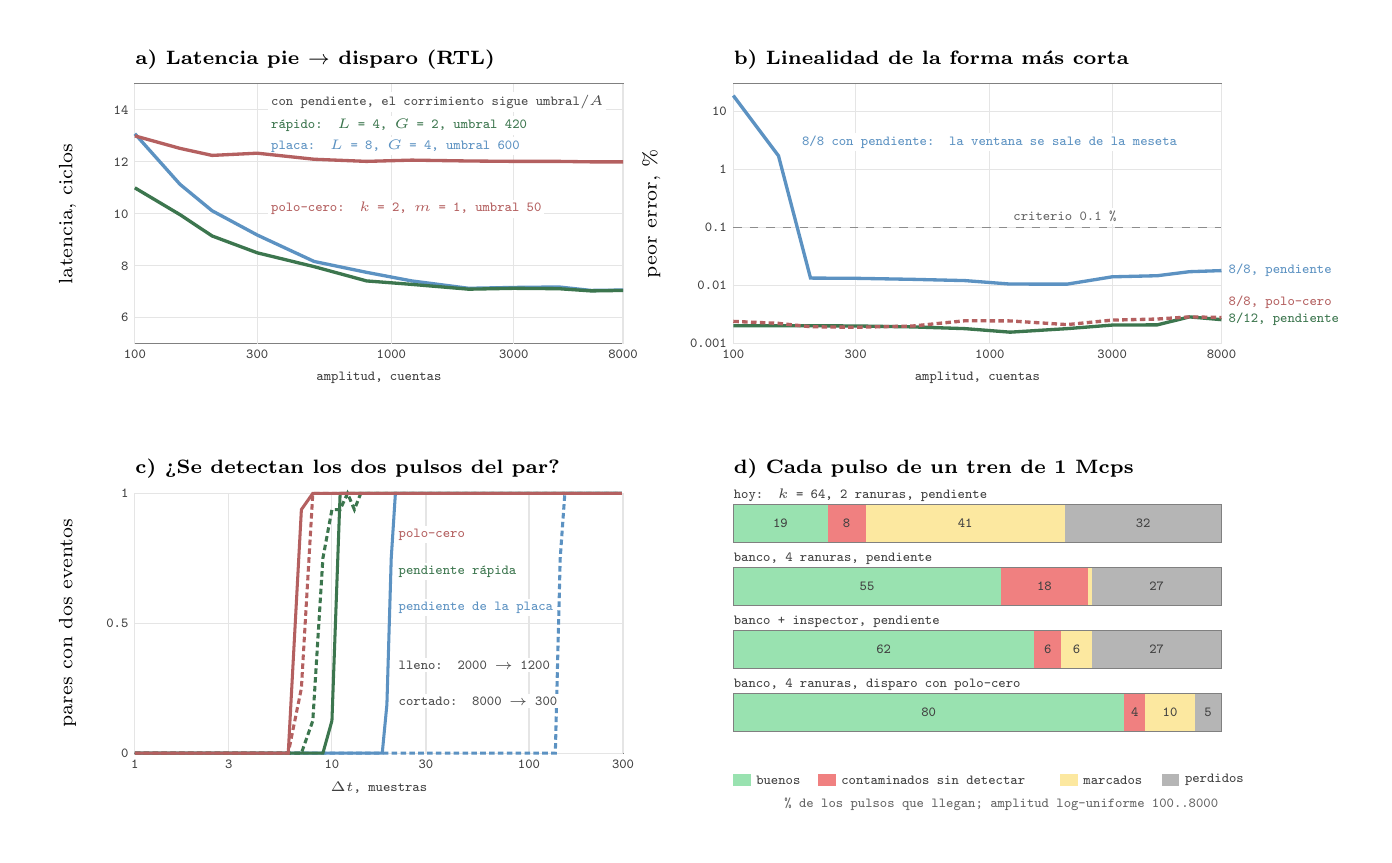
\begin{tikzpicture}[fondo]
\node[anchor=south west, font=\scriptsize\bfseries, inner sep=0pt] at (0.000,8.680) {a) Latencia pie $\to$ disparo (RTL)};
\draw[black!50, line width=0.4pt] (0.000,5.200) rectangle (6.200,8.500);
\draw[black!10] (0.000,5.530) -- (6.200,5.530);
\node[nodo, anchor=east] at (-0.040,5.530) {6};
\draw[black!10] (0.000,6.190) -- (6.200,6.190);
\node[nodo, anchor=east] at (-0.040,6.190) {8};
\draw[black!10] (0.000,6.850) -- (6.200,6.850);
\node[nodo, anchor=east] at (-0.040,6.850) {10};
\draw[black!10] (0.000,7.510) -- (6.200,7.510);
\node[nodo, anchor=east] at (-0.040,7.510) {12};
\draw[black!10] (0.000,8.170) -- (6.200,8.170);
\node[nodo, anchor=east] at (-0.040,8.170) {14};
\draw[black!10] (0.000,5.200) -- (0.000,8.500);
\node[nodo, anchor=north] at (0.000,5.160) {100};
\draw[black!10] (1.554,5.200) -- (1.554,8.500);
\node[nodo, anchor=north] at (1.554,5.160) {300};
\draw[black!10] (3.258,5.200) -- (3.258,8.500);
\node[nodo, anchor=north] at (3.258,5.160) {1000};
\draw[black!10] (4.812,5.200) -- (4.812,8.500);
\node[nodo, anchor=north] at (4.812,5.160) {3000};
\draw[black!10] (6.200,5.200) -- (6.200,8.500);
\node[nodo, anchor=north] at (6.200,5.160) {8000};
\node[nodo, anchor=north] at (3.100,4.880) {amplitud, cuentas};
\node[font=\scriptsize, anchor=south, rotate=90] at (-0.620,6.850) {latencia, ciclos};
\draw[azul!85!black, line width=1.2pt] plot coordinates {(0.000,7.867) (0.574,7.224) (0.981,6.889) (1.554,6.581) (2.277,6.245) (2.942,6.107) (3.516,5.998) (4.239,5.904) (4.812,5.915) (5.386,5.921) (5.793,5.877) (6.200,5.882)};
\node[nodo, anchor=west, text=azul!85!black, fill=white, inner sep=1pt] at (1.689,7.708) {placa: $L$ = 8, $G$ = 4, umbral 600};
\draw[verde!55!black, line width=1.2pt] plot coordinates {(0.000,7.180) (0.574,6.839) (0.981,6.569) (1.554,6.355) (2.277,6.179) (2.942,5.998) (3.516,5.954) (4.239,5.893) (4.812,5.904) (5.386,5.899) (5.793,5.871) (6.200,5.877)};
\node[nodo, anchor=west, text=verde!55!black, fill=white, inner sep=1pt] at (1.689,7.972) {rápido: $L$ = 4, $G$ = 2, umbral 420};
\draw[rojo!75!black, line width=1.2pt] plot coordinates {(0.000,7.840) (0.574,7.681) (0.981,7.592) (1.554,7.620) (2.277,7.543) (2.942,7.516) (3.516,7.532) (4.239,7.521) (4.812,7.516) (5.386,7.516) (5.793,7.510) (6.200,7.510)};
\node[nodo, anchor=west, text=rojo!75!black, fill=white, inner sep=1pt] at (1.689,6.916) {polo-cero: $k$ = 2, $m$ = 1, umbral 50};
\node[nodo, anchor=west, text=black!70, fill=white, inner sep=1pt] at (1.689,8.269) {con pendiente, el corrimiento sigue umbral$/A$};
\node[anchor=south west, font=\scriptsize\bfseries, inner sep=0pt] at (7.600,8.680) {b) Linealidad de la forma más corta};
\draw[black!50, line width=0.4pt] (7.600,5.200) rectangle (13.800,8.500);
\draw[black!10] (7.600,5.200) -- (13.800,5.200);
\node[nodo, anchor=east] at (7.560,5.200) {0.001};
\draw[black!10] (7.600,5.937) -- (13.800,5.937);
\node[nodo, anchor=east] at (7.560,5.937) {0.01};
\draw[black!10] (7.600,6.674) -- (13.800,6.674);
\node[nodo, anchor=east] at (7.560,6.674) {0.1};
\draw[black!10] (7.600,7.411) -- (13.800,7.411);
\node[nodo, anchor=east] at (7.560,7.411) {1};
\draw[black!10] (7.600,8.148) -- (13.800,8.148);
\node[nodo, anchor=east] at (7.560,8.148) {10};
\draw[black!10] (7.600,5.200) -- (7.600,8.500);
\node[nodo, anchor=north] at (7.600,5.160) {100};
\draw[black!10] (9.154,5.200) -- (9.154,8.500);
\node[nodo, anchor=north] at (9.154,5.160) {300};
\draw[black!10] (10.858,5.200) -- (10.858,8.500);
\node[nodo, anchor=north] at (10.858,5.160) {1000};
\draw[black!10] (12.412,5.200) -- (12.412,8.500);
\node[nodo, anchor=north] at (12.412,5.160) {3000};
\draw[black!10] (13.800,5.200) -- (13.800,8.500);
\node[nodo, anchor=north] at (13.800,5.160) {8000};
\node[nodo, anchor=north] at (10.700,4.880) {amplitud, cuentas};
\node[font=\scriptsize, anchor=south, rotate=90] at (6.980,6.850) {};
\node[font=\scriptsize, anchor=south, rotate=90] at (6.800,6.850) {peor error, \%};
\draw[black!45, dashed] (7.600,6.674) -- (13.800,6.674);
\draw[azul!85!black, line width=1.2pt] plot coordinates {(7.600,8.352) (8.174,7.587) (8.581,6.034) (9.154,6.031) (9.877,6.018) (10.542,6.002) (11.116,5.958) (11.839,5.957) (12.412,6.050) (12.986,6.064) (13.393,6.115) (13.800,6.129)};
\draw[verde!55!black, line width=1.2pt] plot coordinates {(7.600,5.429) (8.174,5.429) (8.581,5.428) (9.154,5.426) (9.877,5.414) (10.542,5.392) (11.116,5.347) (11.839,5.392) (12.412,5.437) (12.986,5.440) (13.393,5.541) (13.800,5.506)};
\draw[rojo!75!black, line width=1.2pt, dash pattern=on 2pt off 1.2pt] plot coordinates {(7.600,5.484) (8.174,5.459) (8.581,5.416) (9.154,5.409) (9.877,5.425) (10.542,5.492) (11.116,5.490) (11.839,5.443) (12.412,5.500) (12.986,5.514) (13.393,5.541) (13.800,5.534)};
\node[nodo, anchor=west, text=verde!55!black, inner sep=1pt] at (13.850,5.506) {8/12, pendiente};
\node[nodo, anchor=west, text=rojo!75!black, inner sep=1pt] at (13.850,5.726) {8/8, polo-cero};
\node[nodo, anchor=west, text=azul!85!black, inner sep=1pt] at (13.850,6.129) {8/8, pendiente};
\node[nodo, anchor=west, text=black!60, fill=white, inner sep=1pt] at (11.116,6.825) {criterio 0.1 \%};
\node[nodo, anchor=west, text=azul!85!black, fill=white, inner sep=1pt] at (8.432,7.763) {8/8 con pendiente: la ventana se sale de la meseta};
\node[anchor=south west, font=\scriptsize\bfseries, inner sep=0pt] at (0.000,3.480) {c) ¿Se detectan los dos pulsos del par?};
\draw[black!50, line width=0.4pt] (0.000,0.000) rectangle (6.200,3.300);
\draw[black!10] (0.000,0.000) -- (6.200,0.000);
\node[nodo, anchor=east] at (-0.040,0.000) {0};
\draw[black!10] (0.000,1.650) -- (6.200,1.650);
\node[nodo, anchor=east] at (-0.040,1.650) {0.5};
\draw[black!10] (0.000,3.300) -- (6.200,3.300);
\node[nodo, anchor=east] at (-0.040,3.300) {1};
\draw[black!10] (0.000,0.000) -- (0.000,3.300);
\node[nodo, anchor=north] at (0.000,-0.040) {1};
\draw[black!10] (1.194,0.000) -- (1.194,3.300);
\node[nodo, anchor=north] at (1.194,-0.040) {3};
\draw[black!10] (2.503,0.000) -- (2.503,3.300);
\node[nodo, anchor=north] at (2.503,-0.040) {10};
\draw[black!10] (3.697,0.000) -- (3.697,3.300);
\node[nodo, anchor=north] at (3.697,-0.040) {30};
\draw[black!10] (5.006,0.000) -- (5.006,3.300);
\node[nodo, anchor=north] at (5.006,-0.040) {100};
\draw[black!10] (6.200,0.000) -- (6.200,3.300);
\node[nodo, anchor=north] at (6.200,-0.040) {300};
\node[nodo, anchor=north] at (3.100,-0.320) {$\Delta t$, muestras};
\node[font=\scriptsize, anchor=south, rotate=90] at (-0.620,1.650) {pares con dos eventos};
\draw[azul!85!black, line width=1.1pt] plot coordinates {(0.000,0.000) (0.753,0.000) (1.194,0.000) (1.507,0.000) (1.749,0.000) (1.948,0.000) (2.115,0.000) (2.260,0.000) (2.388,0.000) (2.503,0.000) (2.607,0.000) (2.701,0.000) (2.788,0.000) (2.869,0.000) (2.944,0.000) (3.014,0.000) (3.080,0.000) (3.142,0.000) (3.201,0.619) (3.256,2.475) (3.309,3.300) (3.360,3.300) (3.408,3.300) (3.455,3.300) (3.499,3.300) (3.542,3.300) (3.583,3.300) (3.622,3.300) (3.660,3.300) (3.697,3.300) (3.733,3.300) (3.767,3.300) (3.801,3.300) (3.833,3.300) (3.865,3.300) (3.895,3.300) (3.925,3.300) (3.954,3.300) (3.982,3.300) (4.010,3.300) (4.037,3.300) (4.063,3.300) (4.088,3.300) (4.113,3.300) (4.138,3.300) (4.162,3.300) (4.185,3.300) (4.208,3.300) (4.376,3.300) (4.521,3.300) (4.649,3.300) (4.763,3.300) (4.867,3.300) (4.961,3.300) (5.048,3.300) (5.129,3.300) (5.204,3.300) (5.274,3.300) (5.340,3.300) (5.402,3.300) (5.461,3.300) (5.517,3.300) (5.570,3.300) (5.620,3.300) (5.669,3.300) (5.715,3.300) (5.759,3.300) (5.802,3.300) (5.843,3.300) (5.882,3.300) (5.921,3.300) (5.957,3.300) (5.993,3.300) (6.028,3.300) (6.061,3.300) (6.093,3.300) (6.125,3.300) (6.156,3.300) (6.185,3.300)};
\draw[azul!85!black, line width=1.1pt, dash pattern=on 2pt off 1.2pt] plot coordinates {(0.000,0.000) (0.753,0.000) (1.194,0.000) (1.507,0.000) (1.749,0.000) (1.948,0.000) (2.115,0.000) (2.260,0.000) (2.388,0.000) (2.503,0.000) (2.607,0.000) (2.701,0.000) (2.788,0.000) (2.869,0.000) (2.944,0.000) (3.014,0.000) (3.080,0.000) (3.142,0.000) (3.201,0.000) (3.256,0.000) (3.309,0.000) (3.360,0.000) (3.408,0.000) (3.455,0.000) (3.499,0.000) (3.542,0.000) (3.583,0.000) (3.622,0.000) (3.660,0.000) (3.697,0.000) (3.733,0.000) (3.767,0.000) (3.801,0.000) (3.833,0.000) (3.865,0.000) (3.895,0.000) (3.925,0.000) (3.954,0.000) (3.982,0.000) (4.010,0.000) (4.037,0.000) (4.063,0.000) (4.088,0.000) (4.113,0.000) (4.138,0.000) (4.162,0.000) (4.185,0.000) (4.208,0.000) (4.376,0.000) (4.521,0.000) (4.649,0.000) (4.763,0.000) (4.867,0.000) (4.961,0.000) (5.048,0.000) (5.129,0.000) (5.204,0.000) (5.274,0.000) (5.340,0.000) (5.402,2.475) (5.461,3.300) (5.517,3.300) (5.570,3.300) (5.620,3.300) (5.669,3.300) (5.715,3.300) (5.759,3.300) (5.802,3.300) (5.843,3.300) (5.882,3.300) (5.921,3.300) (5.957,3.300) (5.993,3.300) (6.028,3.300) (6.061,3.300) (6.093,3.300) (6.125,3.300) (6.156,3.300) (6.185,3.300)};
\draw[verde!55!black, line width=1.1pt] plot coordinates {(0.000,0.000) (0.753,0.000) (1.194,0.000) (1.507,0.000) (1.749,0.000) (1.948,0.000) (2.115,0.000) (2.260,0.000) (2.388,0.000) (2.503,0.412) (2.607,3.300) (2.701,3.300) (2.788,3.300) (2.869,3.300) (2.944,3.300) (3.014,3.300) (3.080,3.300) (3.142,3.300) (3.201,3.300) (3.256,3.300) (3.309,3.300) (3.360,3.300) (3.408,3.300) (3.455,3.300) (3.499,3.300) (3.542,3.300) (3.583,3.300) (3.622,3.300) (3.660,3.300) (3.697,3.300) (3.733,3.300) (3.767,3.300) (3.801,3.300) (3.833,3.300) (3.865,3.300) (3.895,3.300) (3.925,3.300) (3.954,3.300) (3.982,3.300) (4.010,3.300) (4.037,3.300) (4.063,3.300) (4.088,3.300) (4.113,3.300) (4.138,3.300) (4.162,3.300) (4.185,3.300) (4.208,3.300) (4.376,3.300) (4.521,3.300) (4.649,3.300) (4.763,3.300) (4.867,3.300) (4.961,3.300) (5.048,3.300) (5.129,3.300) (5.204,3.300) (5.274,3.300) (5.340,3.300) (5.402,3.300) (5.461,3.300) (5.517,3.300) (5.570,3.300) (5.620,3.300) (5.669,3.300) (5.715,3.300) (5.759,3.300) (5.802,3.300) (5.843,3.300) (5.882,3.300) (5.921,3.300) (5.957,3.300) (5.993,3.300) (6.028,3.300) (6.061,3.300) (6.093,3.300) (6.125,3.300) (6.156,3.300) (6.185,3.300)};
\draw[verde!55!black, line width=1.1pt, dash pattern=on 2pt off 1.2pt] plot coordinates {(0.000,0.000) (0.753,0.000) (1.194,0.000) (1.507,0.000) (1.749,0.000) (1.948,0.000) (2.115,0.000) (2.260,0.412) (2.388,2.475) (2.503,3.094) (2.607,3.094) (2.701,3.300) (2.788,3.094) (2.869,3.300) (2.944,3.300) (3.014,3.300) (3.080,3.300) (3.142,3.300) (3.201,3.300) (3.256,3.300) (3.309,3.300) (3.360,3.300) (3.408,3.300) (3.455,3.300) (3.499,3.300) (3.542,3.300) (3.583,3.300) (3.622,3.300) (3.660,3.300) (3.697,3.300) (3.733,3.300) (3.767,3.300) (3.801,3.300) (3.833,3.300) (3.865,3.300) (3.895,3.300) (3.925,3.300) (3.954,3.300) (3.982,3.300) (4.010,3.300) (4.037,3.300) (4.063,3.300) (4.088,3.300) (4.113,3.300) (4.138,3.300) (4.162,3.300) (4.185,3.300) (4.208,3.300) (4.376,3.300) (4.521,3.300) (4.649,3.300) (4.763,3.300) (4.867,3.300) (4.961,3.300) (5.048,3.300) (5.129,3.300) (5.204,3.300) (5.274,3.300) (5.340,3.300) (5.402,3.300) (5.461,3.300) (5.517,3.300) (5.570,3.300) (5.620,3.300) (5.669,3.300) (5.715,3.300) (5.759,3.300) (5.802,3.300) (5.843,3.300) (5.882,3.300) (5.921,3.300) (5.957,3.300) (5.993,3.300) (6.028,3.300) (6.061,3.300) (6.093,3.300) (6.125,3.300) (6.156,3.300) (6.185,3.300)};
\draw[rojo!75!black, line width=1.1pt] plot coordinates {(0.000,0.000) (0.753,0.000) (1.194,0.000) (1.507,0.000) (1.749,0.000) (1.948,0.000) (2.115,3.094) (2.260,3.300) (2.388,3.300) (2.503,3.300) (2.607,3.300) (2.701,3.300) (2.788,3.300) (2.869,3.300) (2.944,3.300) (3.014,3.300) (3.080,3.300) (3.142,3.300) (3.201,3.300) (3.256,3.300) (3.309,3.300) (3.360,3.300) (3.408,3.300) (3.455,3.300) (3.499,3.300) (3.542,3.300) (3.583,3.300) (3.622,3.300) (3.660,3.300) (3.697,3.300) (3.733,3.300) (3.767,3.300) (3.801,3.300) (3.833,3.300) (3.865,3.300) (3.895,3.300) (3.925,3.300) (3.954,3.300) (3.982,3.300) (4.010,3.300) (4.037,3.300) (4.063,3.300) (4.088,3.300) (4.113,3.300) (4.138,3.300) (4.162,3.300) (4.185,3.300) (4.208,3.300) (4.376,3.300) (4.521,3.300) (4.649,3.300) (4.763,3.300) (4.867,3.300) (4.961,3.300) (5.048,3.300) (5.129,3.300) (5.204,3.300) (5.274,3.300) (5.340,3.300) (5.402,3.300) (5.461,3.300) (5.517,3.300) (5.570,3.300) (5.620,3.300) (5.669,3.300) (5.715,3.300) (5.759,3.300) (5.802,3.300) (5.843,3.300) (5.882,3.300) (5.921,3.300) (5.957,3.300) (5.993,3.300) (6.028,3.300) (6.061,3.300) (6.093,3.300) (6.125,3.300) (6.156,3.300) (6.185,3.300)};
\draw[rojo!75!black, line width=1.1pt, dash pattern=on 2pt off 1.2pt] plot coordinates {(0.000,0.000) (0.753,0.000) (1.194,0.000) (1.507,0.000) (1.749,0.000) (1.948,0.000) (2.115,0.825) (2.260,3.300) (2.388,3.300) (2.503,3.300) (2.607,3.300) (2.701,3.300) (2.788,3.300) (2.869,3.300) (2.944,3.300) (3.014,3.300) (3.080,3.300) (3.142,3.300) (3.201,3.300) (3.256,3.300) (3.309,3.300) (3.360,3.300) (3.408,3.300) (3.455,3.300) (3.499,3.300) (3.542,3.300) (3.583,3.300) (3.622,3.300) (3.660,3.300) (3.697,3.300) (3.733,3.300) (3.767,3.300) (3.801,3.300) (3.833,3.300) (3.865,3.300) (3.895,3.300) (3.925,3.300) (3.954,3.300) (3.982,3.300) (4.010,3.300) (4.037,3.300) (4.063,3.300) (4.088,3.300) (4.113,3.300) (4.138,3.300) (4.162,3.300) (4.185,3.300) (4.208,3.300) (4.376,3.300) (4.521,3.300) (4.649,3.300) (4.763,3.300) (4.867,3.300) (4.961,3.300) (5.048,3.300) (5.129,3.300) (5.204,3.300) (5.274,3.300) (5.340,3.300) (5.402,3.300) (5.461,3.300) (5.517,3.300) (5.570,3.300) (5.620,3.300) (5.669,3.300) (5.715,3.300) (5.759,3.300) (5.802,3.300) (5.843,3.300) (5.882,3.300) (5.921,3.300) (5.957,3.300) (5.993,3.300) (6.028,3.300) (6.061,3.300) (6.093,3.300) (6.125,3.300) (6.156,3.300) (6.185,3.300)};
\node[nodo, anchor=west, text=rojo!75!black, fill=white, inner sep=1pt] at (3.309,2.772) {polo-cero};
\node[nodo, anchor=west, text=verde!55!black, fill=white, inner sep=1pt] at (3.309,2.310) {pendiente rápida};
\node[nodo, anchor=west, text=azul!85!black, fill=white, inner sep=1pt] at (3.309,1.848) {pendiente de la placa};
\node[nodo, anchor=west, text=black!70, fill=white, inner sep=1pt] at (3.309,1.122) {lleno: 2000 $\to$ 1200};
\node[nodo, anchor=west, text=black!70, fill=white, inner sep=1pt] at (3.309,0.660) {cortado: 8000 $\to$ 300};
\node[anchor=south west, font=\scriptsize\bfseries, inner sep=0pt] at (7.600,3.480) {d) Cada pulso de un tren de 1 Mcps};
\node[nodo, anchor=south west, inner sep=0pt] at (7.600,3.190) {hoy: $k$ = 64, 2 ranuras, pendiente};
\fill[verde!70] (7.600,2.680) rectangle (8.797,3.160);
\node[nodo] at (8.198,2.920) {19};
\fill[rojo] (8.797,2.680) rectangle (9.280,3.160);
\node[nodo] at (9.038,2.920) {8};
\fill[amarillo] (9.280,2.680) rectangle (11.812,3.160);
\node[nodo] at (10.546,2.920) {41};
\fill[grisr!80!black] (11.812,2.680) rectangle (13.800,3.160);
\node[nodo] at (12.806,2.920) {32};
\draw[black!50, line width=0.3pt] (7.600,2.680) rectangle (13.800,3.160);
\node[nodo, anchor=south west, inner sep=0pt] at (7.600,2.390) {banco, 4 ranuras, pendiente};
\fill[verde!70] (7.600,1.880) rectangle (10.999,2.360);
\node[nodo] at (9.299,2.120) {55};
\fill[rojo] (10.999,1.880) rectangle (12.103,2.360);
\node[nodo] at (11.551,2.120) {18};
\fill[amarillo] (12.103,1.880) rectangle (12.154,2.360);
\fill[grisr!80!black] (12.154,1.880) rectangle (13.800,2.360);
\node[nodo] at (12.977,2.120) {27};
\draw[black!50, line width=0.3pt] (7.600,1.880) rectangle (13.800,2.360);
\node[nodo, anchor=south west, inner sep=0pt] at (7.600,1.590) {banco + inspector, pendiente};
\fill[verde!70] (7.600,1.080) rectangle (11.421,1.560);
\node[nodo] at (9.510,1.320) {62};
\fill[rojo] (11.421,1.080) rectangle (11.766,1.560);
\node[nodo] at (11.593,1.320) {6};
\fill[amarillo] (11.766,1.080) rectangle (12.154,1.560);
\node[nodo] at (11.960,1.320) {6};
\fill[grisr!80!black] (12.154,1.080) rectangle (13.800,1.560);
\node[nodo] at (12.977,1.320) {27};
\draw[black!50, line width=0.3pt] (7.600,1.080) rectangle (13.800,1.560);
\node[nodo, anchor=south west, inner sep=0pt] at (7.600,0.790) {banco, 4 ranuras, disparo con polo-cero};
\fill[verde!70] (7.600,0.280) rectangle (12.563,0.760);
\node[nodo] at (10.082,0.520) {80};
\fill[rojo] (12.563,0.280) rectangle (12.833,0.760);
\node[nodo] at (12.698,0.520) {4};
\fill[amarillo] (12.833,0.280) rectangle (13.461,0.760);
\node[nodo] at (13.147,0.520) {10};
\fill[grisr!80!black] (13.461,0.280) rectangle (13.800,0.760);
\node[nodo] at (13.630,0.520) {5};
\draw[black!50, line width=0.3pt] (7.600,0.280) rectangle (13.800,0.760);
\fill[verde!70] (7.600,-0.420) rectangle ++(0.22,0.16);
\node[nodo, anchor=west] at (7.850,-0.340) {buenos};
\fill[rojo] (8.680,-0.420) rectangle ++(0.22,0.16);
\node[nodo, anchor=west] at (8.930,-0.340) {contaminados sin detectar};
\fill[amarillo] (11.755,-0.420) rectangle ++(0.22,0.16);
\node[nodo, anchor=west] at (12.005,-0.340) {marcados};
\fill[grisr!80!black] (13.045,-0.420) rectangle ++(0.22,0.16);
\node[nodo, anchor=west] at (13.295,-0.340) {perdidos};
\node[nodo, anchor=north east, text=black!60] at (13.800,-0.520) {\% de los pulsos que llegan; amplitud log-uniforme 100..8000};
\end{tikzpicture}
\end{document}
